\documentclass[10pt]{article}
\usepackage[utf8]{inputenc}
\usepackage{parskip}
\usepackage[margin = 1in]{geometry}
\usepackage{xcolor}
\usepackage[colorlinks = true,linkcolor = blue, urlcolor  = blue,citecolor = blue,anchorcolor = blue]{hyperref}
\usepackage{framed}
\usepackage{apacite}
\usepackage[authoryear,sort]{natbib}
\usepackage{amsmath}
\usepackage{amssymb}
\bibliographystyle{apalike}
\newcommand{\E}{\textrm{E}}
\newcommand\bref[2]{\href{#1}{\color{blue}{#2}}}
\renewcommand*{\theenumi}{\thesection.\arabic{enumi}}
\renewcommand{\P}{\text{P}}
\usepackage{tikz}
\usetikzlibrary{arrows,shapes.arrows,positioning,shapes,patterns,calc}

\begin{document}

\begin{Large} 
Info 6751. Fall 2022. Problem Set 13. Due on Canvas by 5pm on 29 Nov (Tuesday deadline to avoid the day immediately after break).
\end{Large}
\hline \vskip .1in

\section{(30 points) Instrumental variables in experiments}

Suppose you are an elementary school principal. You randomize some students to a new program to receive extra tutoring at an off-site location in the evenings. You randomize other students to a no-tutoring condition.

\begin{center}
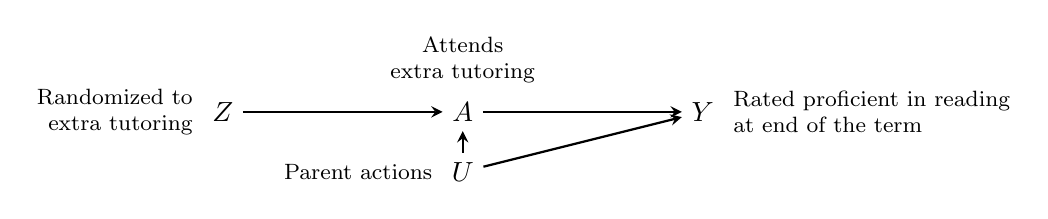
\begin{tikzpicture}[x = .3in, y = .15in]
    \node (z) at (-6,0) {$Z$};
    \node (a) at (-2,0) {$A$};
    \node (y) at  (2,0) {$Y$};
    \node[font = \footnotesize, align = right, anchor = east] at (z.west) {Randomized to\\extra tutoring};
    \node (u) at  (-2,-2) {$U$};
    \node[font = \footnotesize, align = center, anchor = south] at (a.north) {Attends\\extra tutoring};
    \node[font = \footnotesize, align = left, anchor = west] at  (y.east) {Rated proficient in reading\\at end of the term};
    \node[font = \footnotesize, align = right, anchor = east] at (u.west) {Parent actions};
    \draw[->, >=stealth, thick] (z) -- (a);
    \draw[->, >=stealth, thick] (a) --  (y);
    \draw[->, >=stealth, thick] (u) --  (a);
    \draw[->, >=stealth, thick] (u) --  (y);
  \end{tikzpicture}
\end{center}

In many cases, students' treatment assignments $Z$ determines their actual treatments $A$ (when $Z = 1$ then $A = 1$, and when $Z = 0$ then $A = 0$). But there are some difficulties:
\begin{itemize}
\item[a)] The parents of some students work evenings and can't drive their children to the tutoring ($U$). No matter the value of $Z$, these children do not receive tutoring ($A = 0$).
\item[b)] The parents of some students make a huge fuss ($U$) so that regardless of the value of $Z$, these parents ensure that their children receive tutoring ($A = 1$).
\end{itemize}

Using the terms discussed in class,

\begin{enumerate}
\item (5 points) What is the intent to treat effect (in words)?
\item (5 points) Who are the always-takers?
\item (5 points) Who are the never-takers?
\item (5 points) Who are the compliers?
\item (5 points) Although they are not discussed above, describe how someone could be a defier.
\item (5 points) What assumption was made credible by randomization of $Z$?
\end{enumerate}

\section{(20 points) Instrumental variables in observational studies}

Much of the water supply for the state of California comes from snowmelt in the Sierra Nevada Mountains. Two economists are very excited to notice that some years have much larger snowpacks than others---this could be an instrument!

\begin{table}[!ht]
\centering
\begin{tabular}{c : c}
  Economist 1 & Economist 2 \\
  \hline
  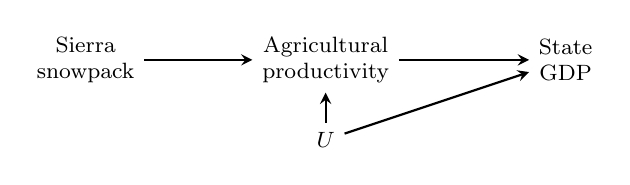
\begin{tikzpicture}[x = .3in, y = .2in]
    \node[font = \footnotesize, align = center] (z) at (-6,0) {Sierra\\snowpack};
    \node[font = \footnotesize, align = center] (t) at (-2,0) {Agricultural\\productivity};
    \node[font = \footnotesize, align = center] (y) at  (2,0) {State\\GDP};
    \node[font = \footnotesize] (u) at  (-2,-2) {$U$};
    \draw[->, >=stealth, thick] (z) -- (t);
    \draw[->, >=stealth, thick] (t) --  (y);
    \draw[->, >=stealth, thick] (u) --  (t);
    \draw[->, >=stealth, thick] (u) --  (y);
  \end{tikzpicture} &
  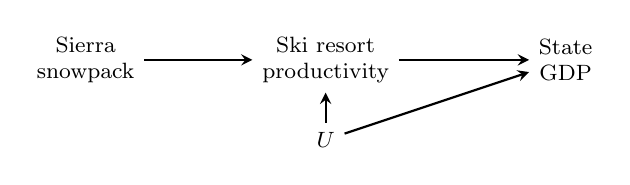
\begin{tikzpicture}[x = .3in, y = .2in]
    \node[font = \footnotesize, align = center] (z) at (-6,0) {Sierra\\snowpack};
    \node[font = \footnotesize, align = center] (t) at (-2,0) {Ski resort\\productivity};
    \node[font = \footnotesize, align = center] (y) at  (2,0) {State\\GDP};
    \node[font = \footnotesize] (u) at  (-2,-2) {$U$};
    \draw[->, >=stealth, thick] (z) -- (t);
    \draw[->, >=stealth, thick] (t) --  (y);
    \draw[->, >=stealth, thick] (u) --  (t);
    \draw[->, >=stealth, thick] (u) --  (y);
  \end{tikzpicture}
\end{tabular}
\end{table}

The first economist argues that random differences in the Sierra snowpack create random fluctuations in agricultural productivity, thereby providing an instrumental variable for the effect of agricultural productivity on the state's GDP.

The second economist argues that random difference in the Sierra snowpack create random fluctuations in the quality of skiing at Mammoth Mountain and other Sierra resorts, thereby providing an instrumental variable for the effect of ski resort productivity on the state's GDP.

\begin{enumerate}
\item (20 points) Both economists argue that their instruments are valid because the snowpack is randomly assigned. Can both economists be right that their instrument is valid? Why or why not?
\end{enumerate}





\end{document}

